\section{Introduction}
%Commonsense knowledge is an important ingredient in machine comprehension and
%inference. 
Intelligent systems about comprehension and inference 
can be improved by incorporating commonsense knowledge as background, 
such as ice is cold, 
chewing is a subevent of eating, 
chair and table are typically found near each other, etc. 
Such commonsense facts could benefit entailment~\cite{dagan2009recognizing}, grounded entailment~\cite{bowman2015large}, or visual recognition tasks~\cite{zhu2014reasoning}.
Such commonsense knowledge is often represented as relation triples
between two concepts or objects in ConceptNet,
which is largely manually curated
or crowd-sourced by community efforts, and thus does not scale well.
For example, ConceptNet\footnote{\url{http://conceptnet.io/}} by MIT \cite{speer2012representing}, one of the largest commonsense
knowledge graph available today, contains only 49 \lnear~
relation triples. 
%Many commonly co-located objects such as (house, garden) and 
%(fork, knife) are not included in this knowledge base. 
Another problem is that such commonsense knowledge bases are typically contributed by just a very limited number of people due to the cost of manual labor. 
Thus no meaningful statistical scores can be
associated with the triples, making rank-based 
computation difficult. 
%For instance, although ConceptNet gives a confidence
%score (from 0 to infinity) to each triple, most of the triples have the default
%score of 1, simply because the human contributor did not or could not 
%provide a score. 
%If such commonsense knowledge is harnessed automatically
%from open-domain text corpora, both of the above problems can be 
%effectively addressed. 
%Open information extraction not only provides the much needed scale,
%but also valuable statistics that can turn into confidence scores.
%
\begin{figure}[th]
\center
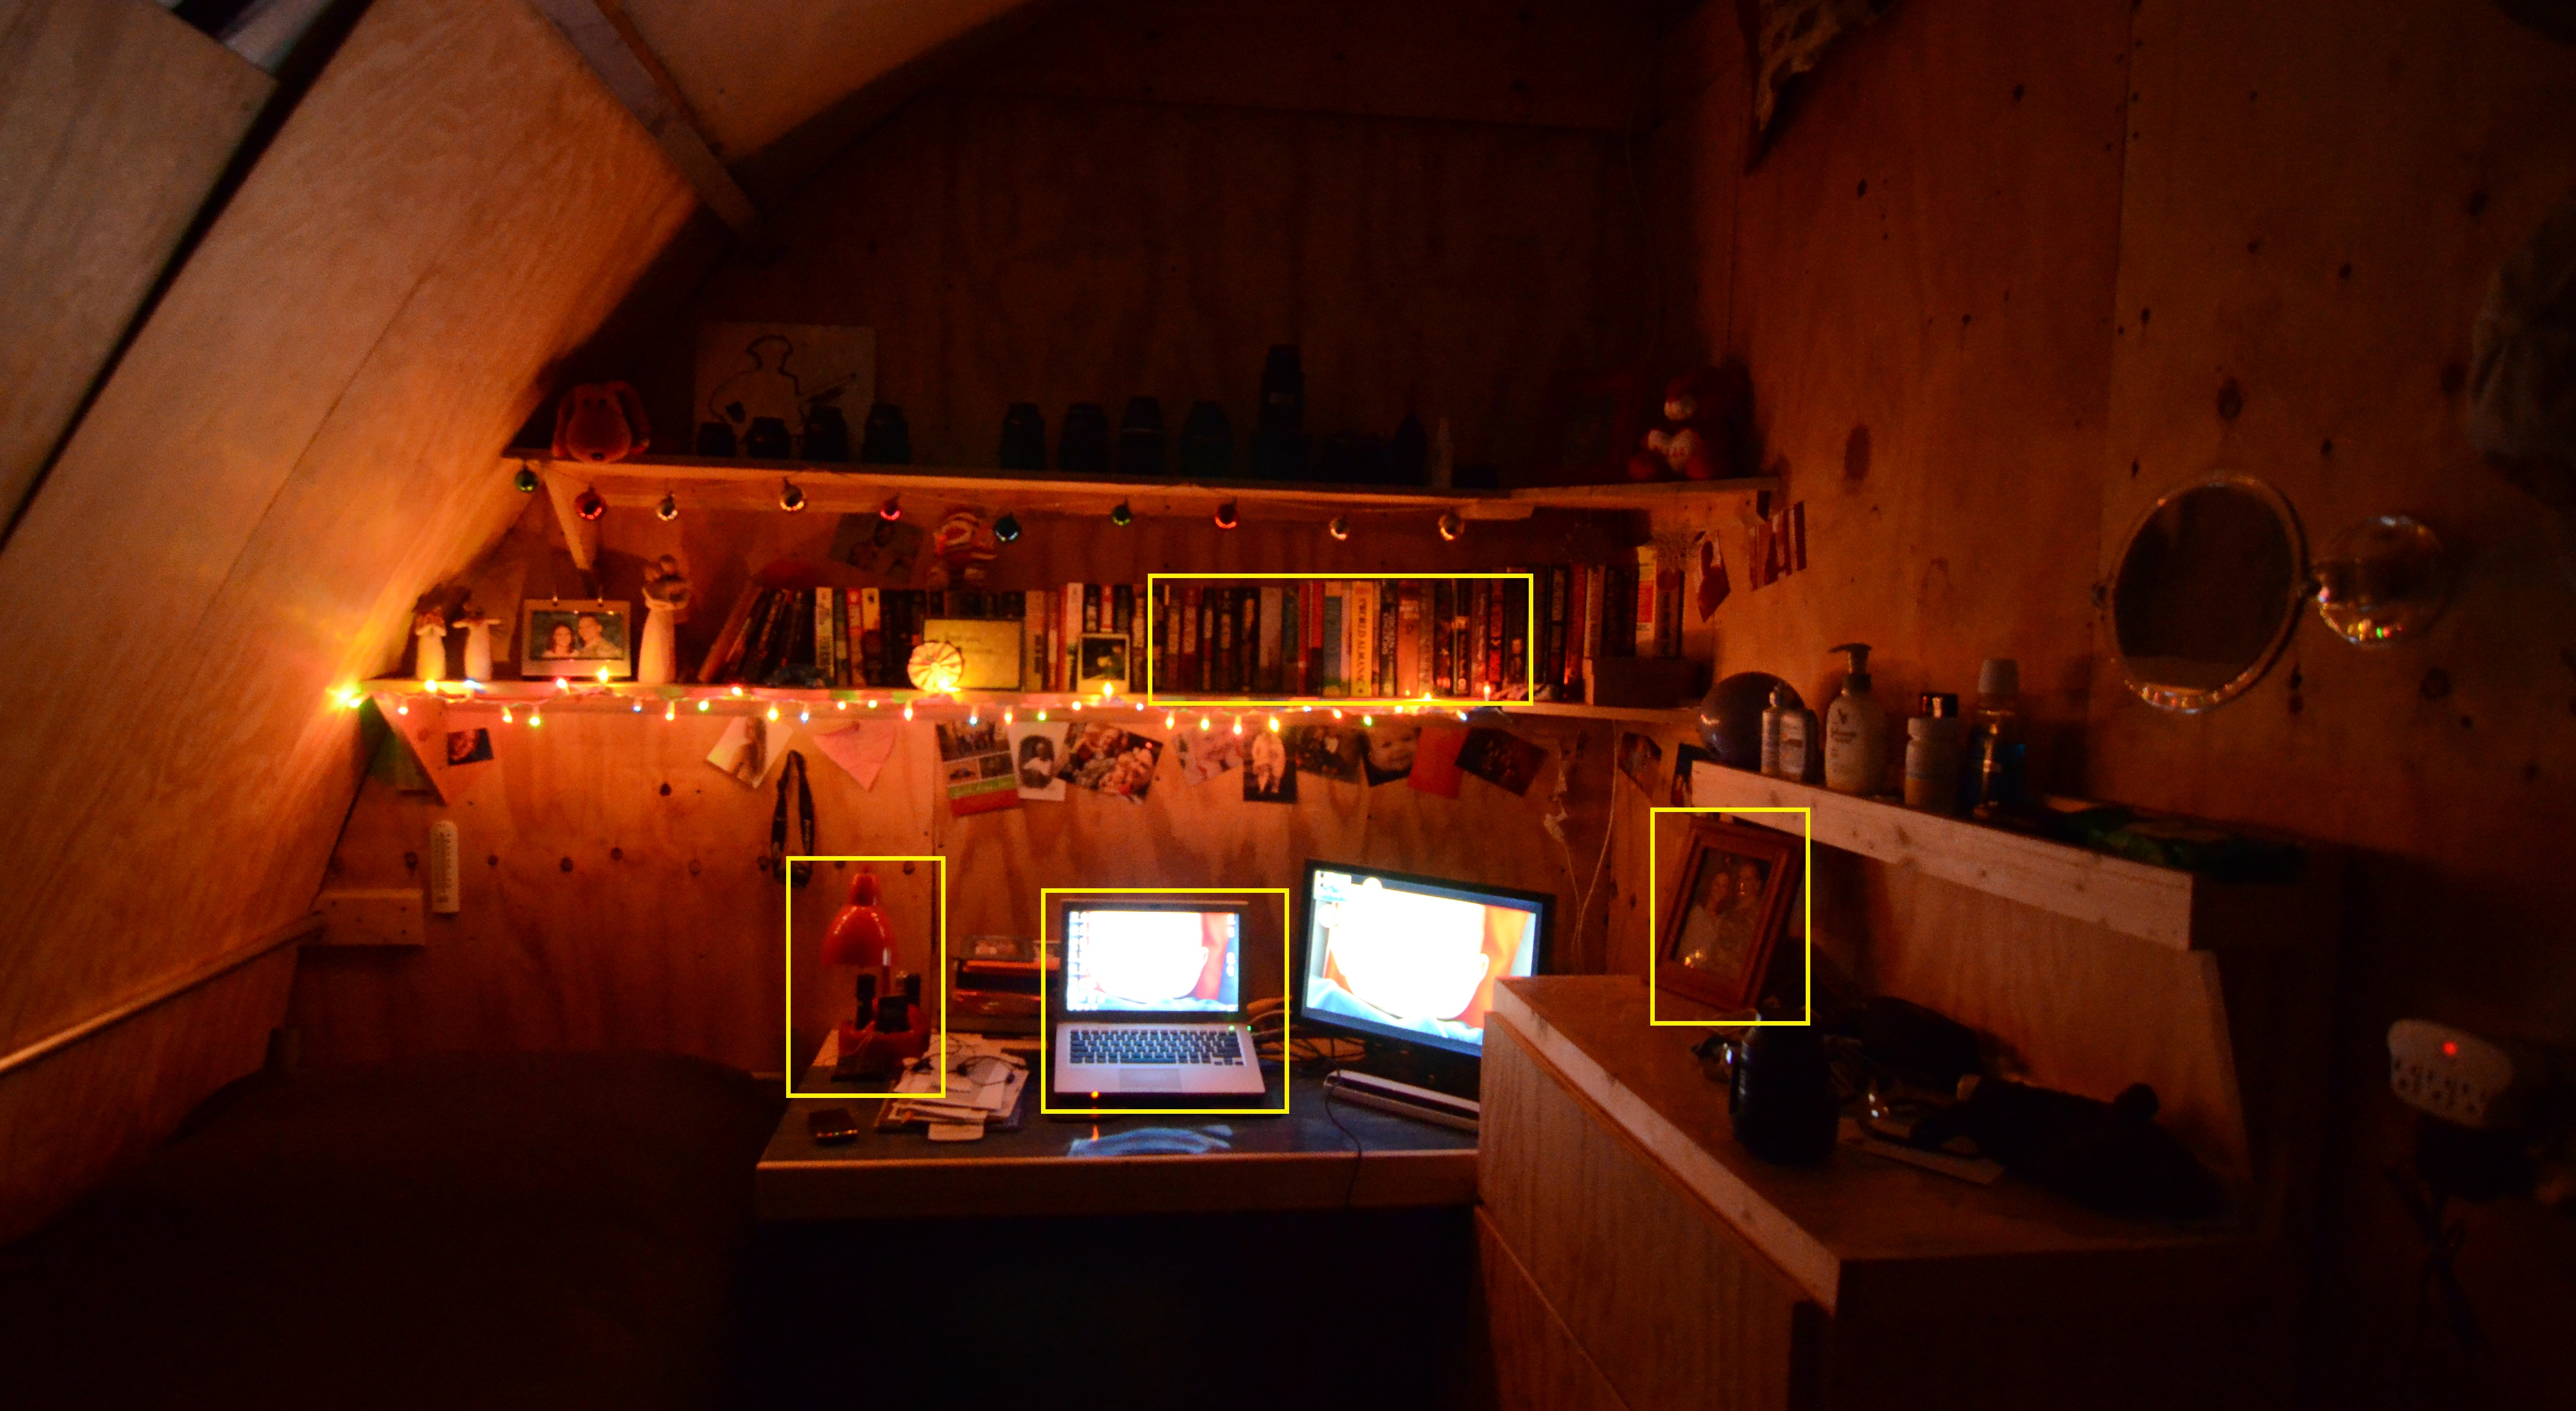
\includegraphics[width=0.9\columnwidth]{dim-room.jpg}
\caption{A dimly lit room with a working table setting, a bright laptop and a dim lamp, photo frame and books}
\label{fig:dim}
\end{figure}

Our goal is to extract the \lnear\ relation between
physical objects, which is defined as two objects typically found near each
other.
%\footnote{Because some physical objects can be a location itself, this
%relation may include some instances of the \textsc{atLocation} relation,
%e.g., {\em room} and {\em door}.}
We focus on \lnear\ relation for these reasons: 
i) such prior knowledge of \lnear\ relations is helpful for 
object detection in complex image 
scenes. 
For example, in a dimly lit room with settings shown in \figref{fig:dim}, if a bright laptop are present on a table,
one may guess that the lamp, photo frame and books maybe nearby based on his/her commonsense knowledge, 
even though these objects are hardly visible due to the low light. 
%(The guess can be based on commonsense knowledge learned from room settings scene description in articles and texts.)
%Such prior knowledge helps with the object detection accuracy; 
ii) \lnear~ relation can benefit general reasoning in reading comprehension,
question answering and many other AI tasks;
iii) existing knowledge bases such as ConceptNet have very limited facts for
this relation.

%
%\begin{enumerate}
%\item \lnear relation is useful for object detection in complex image 
%scenes. For example, in a dimly lit room with a dining table and some chairs.
%One may guess that plates and other kitchenware maybe present on the table.
%Such prior knowledge helps with the object detection accuracy. \KZ{give a 
%real image here which is hard to detect by state-of-the-art algo but 
%obeys commonsense.}
%
%%\item \lnear relation can also be useful for automated conversation systems
%%where meaningful context maybe added to the conversation. \KZ{Example?}
%
%\item \lnear relation can benefit general reasoning in reading comprehension,
%question answering and many other AI tasks.
%
%\item Existing knowledge bases such as Concept Net has very limited facts for
%this relation.
%\end{enumerate}

%Automatic extraction of relations from open text has a short but rich history. 
%Attempts have been made to extract isA, causal, correlation, and 
%also open domain relations (e.g., ReVerb, Yago).
%%\KZ{cite and Say more about KBC}. 
%\lnear~relation is unique and poses significant challenges
%for the following reasons:
%
%i) It involves physical (often visible) objects whereas other 
%popular relations involve general concepts or just natural language terms. 
%
%ii) The distribution of \lnear~ relation is not even across domains: 
%it is more prevalent in literary work such as stories 
%and dramas which come with descriptive scenes rather
%than in news, science \& technology related articles or online user 
%generated content. 
%%Our preliminary investigation shows that XXX\% of the sentences 
%%in New York Times and YYY\% of the sentences
%%in Wikipedia contains a \lnear~ relation, 
%%while that percentage for novels and stories in Gutenberg corpus is ZZZ\%. 
%
%iii) Sentences in literature are often complex and nuanced, 
%which makes extraction particularly challenging. Consider the objects
%``bed'' and ``star'' in the following
%sentence: ``{\em Until at last all the promenaders had gone home to bed, 
%and I was alone with the star.}'' Bed is not near the star
%because it's at another location.
%
%iv) Labeling such sentence is a non-trivial task, 
%and obtaining a large training set is difficult and expensive.
%
%\BL{add more related work about KBC here, mainly about Xiang Li (TTIC) and Stating the Obvious; to stress that why we are using raw text}

%Since raw text of novels tend to contain many 
%descriptions of  scene in real life, 
%we argue that it is feasible to obtain unseen 
%{\lnear} relations from raw novel text. 

In this paper we propose two tasks in solving \lnear\ relation
extraction problem. 
One is a binary classification problem which judges whether 
a sentence describing two physical objects is describing \lnear\ relation between them.
The other is given results of the above classification on a
large number of sentences, how to produce a ranked list of \lnear\
facts as a knowledge base.
Notice that two objects that are {\em co-located} in a couple of sentences
may not mean they have the \lnear\ relation as commonsense.
To this end, we created two 
benchmark datasets: one has 5,000 sentences, 
each describing a scene of two physical objects,
and a label indicating the two objects are co-located in this scene or not; 
the other consists of 500 pairs of
objects with binary labels indicating whether a pair is \lnear\ or not according to commonsense knowledge.  

%is to build a framework to automatically extract 
%large amount of unseen object pairs with \lnear relations 
%from literary text corpora.
%that 
%are not already included in ConceptNet. \KZ{Need to back up this claim in eval}
%Considering the fact that not all sentences mentioning two physical objects 
%indicate that the two objects are nearby each other, 
%our proposed approach is to first construct a sentence-level relation classification model 
%to identify \lnear~ relation and then score each candidate object pair with the model 
%and the sentences containing it.
%Thus, the core problem is to judge whether a given sentence 
%containing two objects is describing a \lnear~ relation between the two objects or not. 
%

%More formally, given a sentence $s$ mentioning a pair of physical objects 
%\textless$e_1,e_2$\textgreater, 
%the problem is to determine whether $e_1$ and $e_2$ are located near each other in a physical scene 
%described in the sentence $s$. 
%
%\begin{table}[th!]
%	\centering
%	\caption{Examples for sentence-level \lnear Classification; The  \textless$e_1,e_2$\textgreater in both instances is \textless dog,cat\textgreater. Since the the first sentence is describing a physical scene about the dog and the cat, 
%		while the dog and the cat in the second sentence do not have to be located near since it is just talking about a general comparison.}
%	\label{tbl:lnc}
%	\begin{tabular}{|c|c|}
%		\hline
%		$s$    &  T/F\\ \hline
%	My dog is older than her cat.	 &  T\\ \hline
%	The King put his dog and cat on the table.     & F  \\ \hline
%	\end{tabular}
%
%\end{table}
%
%\KZ{Can use the two examples earlier. 
%For example, suppose $s_1$ = ``The King put his dog and cat on the table.'', 
%$s_2$ = ``My dog is older than her cat.'', 
%$e_1$ is ``dog" and $e_2$ is ``cat''. 
%Then the answer of $s_1$ is \textit{True} and of  $s_2$ is \textit{False} , 
%since the $s_1$ is describing a physical scene about the dog and the cat, 
%while the dog and the cat in $s_2$ do not have to be located near since it is just talking about a general comparison.
%}

%\BL{Add related work here about the relation classification , and their shortcoming (too many parameters) }

We also propose two kinds of baseline methods to solve the classification task.
The first approach leverages syntactic features and word embedding
in the sentence in a SVM model. 
The second approach is a LSTM
model that takes advantage of word embeddings of the 
two objects and the most relevant sequential information of the sentences 
indicating the co-location, significantly reducing the size of 
parameters. 
We associate a probabilistic score with each object pair,
and then aggregate such scores for each unique pair,
to produce a commonsense knowledge score for this pair.  
%We construct a dataset consisting of \BL{xxx} instances with labels 
%(\textit{True}/\textit{False}) for training our model. 
%Experiments demonstrate that both of the classification methods 
%outperforms the state-of-art approaches on the \lnear dataset.
%\KZ{Need to back up these in the eval.} 

In summary, this paper makes the following contributions:
\begin{itemize}
	\item We propose two novel tasks for \lnear~ relation extraction
	(\secref{sec:method}).
	\item We make public the first annotated dataset for 
	sentence-level \lnear~ relation classification and another dataset for
	\lnear~ knowledge construction (\secref{sec:data}). 
	%	\item We propose a bootstrapping framework that automatically generate X times more training data than the initially labeled.	
	\item We suggest several baseline methods for \lnear~ relation 
	classification task (\secref{sec:method}), 
	which compare favorably with the current state-of-the-art
	method for general-purpose relation classification problem (\secref{sec:eval}). 
	
	\item We extract in total 2,067 new pairs previous not in
	ConceptNet, with a precision of 0.68 (\secref{sec:eval}).
\end{itemize}


